% !TEX root = main.tex
\chapter[head={\CP violation in the $B$-meson sector},tocentry={$\symbfsf{C{}P}$ violation in the $\symbfsf{B}$-meson sector}]
{$\symbfsf{C{}P}$ violation in the $\symbfsf{B}$-meson sector}
\label{chap:CPV}

According to the $CPT$ theorem \CP violation is equivalent to $T$ violation. As described in \cref{sec:symmetriesInSM} the $T$ operator
is antiunitary and therefore transforms numbers into their complex conjugate.
Hence the \CP transformation also affects the complex phases of the bras and kets describing arbitrary initial and final states.
The absolute values of those phases are not physically meaningful as they can be rephased at will.
The physical meaningful quantities are the relative phase differences between coherent contributions to a transition, as these are invariant under global rephasings.
There are three types of transition amplitudes: Weak phases change sign under \CP transformation (\CP-odd) while strong phases do not change sign under \CP transformation (\CP-even).
Spurious phases usually arise due to conventional rephasings and for convenience will be set to zero in the following .
Also it may be noted, that the denotations 'weak' and 'strong' do not mean that the phases originate in weak or strong interactions, but only describe their behaviour under \CP transformation.

This chapter describes first the time evolution of neutral mesons by example of uncharged \B-mesons before discussing the three classes of \CP violation.
More details can be found in Refs.~\cite{Branco:396964,Bigi:1295518}


\section[head={Time evolution of neutral \B-mesons},tocentry={Time evolution of neutral $\symbfsf{\B}$-mesons}]{Time evolution of neutral $\symbfsf{\B}$-mesons}
\label{sec:TimeEvolution}

As explained in \cref{sec:unitarityTriangle} the mass eigenstates and the eigenstates to the weak interaction are not identical for
quarks. The same holds for bound states of quarks like \B-mesons. Studying the system of a \Bz (\bquarkbar\dquark) and a \Bzb-meson
(\bquark\dquarkbar), the most general description to deduce the time evolution is the Schrödinger equation:
\begin{equation}
i\frac{d}{dt}\begin{pmatrix} \Bz \\ \Bzb \end{pmatrix} = H \begin{pmatrix} \Bz \\ \Bzb \end{pmatrix}
=\left(M-\frac{i}{2}\Gamma\right)\begin{pmatrix} \Bz \\ \Bzb \end{pmatrix},
\end{equation}
with the hermitian 2x2 matrices $M$ and $H$ where $m_{11}=m_{22}\equiv m$, $\Gamma_{11}=\Gamma_{22}\equiv\Gamma$, $m_{12}=m_{21}^\ast$ and $\Gamma_{12}=\Gamma_{21}^\ast$ due to the $CPT$ theorem.
The matrix $M$ describes virtual off-shell contributions to the transitions, while the matrix $\Gamma$ real physical states describe to which \Bz and \Bzb decay.
For both matrices the diagonal elements of this matrix express transitions with quantum number transitions $\Delta F=1$ while the off diagonal elements are responsible for quantum number transitions with $\Delta F=2$.
These $\Delta F=2$ processes describe transitions between particles and their correspondiog antiparticle.
The Feynman graphs of lowest order are shown in \cref{fig:FeynmanMixing}.
\begin{figure}[tbp]
	\centering
	\includestandalone{03CPV/figs/Bmixing_1}
	\hspace{0.5cm}
	\includestandalone{03CPV/figs/Bmixing_2}
	\caption{Box diagrams of lowest order for the \Bz-\Bzb-oscillation. Both diagrams are dominated by the \tquark-quark \cite{Ellis:2016jkw}.}
	\label{fig:FeynmanMixing}
\end{figure}
Diagonalising the matrix leads to the masses and widths of the mass eigenstates.
In the \Bz-meson system these are denoted with $\B_H$ and $\B_L$ referring to the heavier and lighter eigenstate, respectively.
The eigenvalues are
\begin{equation}
\begin{split}
\mu_H &= m_H-\frac{i}{2}\Gamma_H = m + \mathcal{Re}\left(F\right)-\frac{i}{2}\left(\Gamma-2\mathcal{Im}\left(F\right)\right)\\
\mu_L &= m_L-\frac{i}{2}\Gamma_L = m - \mathcal{Re}\left(F\right)-\frac{i}{2}\left(\Gamma+2\mathcal{Im}\left(F\right)\right)\label{eq:Mass_eigenvalues}
\end{split}
\end{equation}
with
\begin{equation}
F=\sqrt{\left(m_{12}-\frac{i}{2}\Gamma_{12}\right)\left(m_{12}^\ast-\frac{i}{2}\Gamma_{12}^\ast\right)}.
\end{equation}
The eigenstates can be expressed as
\begin{equation}
\begin{split}
\left|B_H\right>&\sim p\left|\Bz\right>-q\left|\Bzb\right>\\
\left|B_L\right>&\sim p\left|\Bz\right>+q\left|\Bzb\right>\label{eq:Mass_eigenstates}
\end{split}
\end{equation}
where $p$ and $q$ by construction are constrained to fulfil $\left|p\right|^2+\left|q\right|^2=1$.
The ratio $\frac{q}{p}$ can also be expressed in terms of the matrix elements:
\begin{equation}
\frac{q}{p}=\sqrt{ \frac{ m_{12}^\ast-\frac{i}{2}\Gamma_{12}^\ast }{ m_{12}-\frac{i}{2}\Gamma_{12} }}
=\frac{\dm-\frac{i}{2}\DG}{2\left(m_{12}-\frac{i}{2}\Gamma_{12}\right)}\label{eq:qoverp}
\end{equation}
The masses and widths of the initial states can be expressed as
\begin{equation}
m=\frac{m_L+m_H}{2}\hspace{0.5cm}\text{and}\hspace{0.5cm}\Gamma=\frac{\Gamma_L+\Gamma_H}{2}
\end{equation}
while the corresponding differences will be referred to as
\begin{equation}
\dm=m_H-m_L\hspace{0.5cm}\text{and}\hspace{0.5cm}\DG=\Gamma_L-\Gamma_H.
\end{equation}
Using the eigenstates from \cref{eq:Mass_eigenstates} and eigenvalues from \cref{eq:Mass_eigenvalues} the Schrödinger equation can be rewritten as
\begin{equation}
i\frac{d}{dt}\begin{pmatrix} B_L \\ B_H \end{pmatrix} = \begin{pmatrix} \mu_L & 0 \\ 0 & \mu_H \end{pmatrix}\begin{pmatrix} B_L \\ B_H \end{pmatrix},
\end{equation}
which can be easily solved and leads to the time evolution of the mass eigenstates with simple exponential functions $B_{L,H}=e^{-i\mu_{L,H}t}B_{L,H}$.
Reverting \cref{eq:Mass_eigenstates} the time evolution for the flavour eigenstates follows straightforward:
\begin{equation}
\begin{split}
\left|\Bz\!\left(t\right)\right>&=\left|\Bz\right>g_+-\frac{q}{p}\left|\Bzb\right>g_-\\
\left|\Bzb\!\left(t\right)\right>&=\left|\Bzb\right>g_--\frac{p}{q}\left|\Bz\right>g_+ \label{eq:timeEvolution}
\end{split}
\end{equation}
with $g_\pm=\frac{1}{2}\left(e^{-i\mu_Ht}\pm e^{-i\mu_Lt}\right)$.

\section[head={Types of \CP violation},tocentry={Classes of \CP violation}]{Classes of $\symbfsf{C{}P}$ violation}
\label{sec:CPVClasses}

As described in \cref{sec:symmetriesInSM} the the \CP symmetry is broken by the weak interaction.
Further, as explained at the beginning of the chapter \CP affects the complex phases of the corresponding transitions.
For this first the transitions shall be distinguished by the change in internal quantum number $N_q$ and assigned to the matrix elements of $H$.
The digaonal matrix elements describe transitions with $\Delta F=1$, \ie pure decays, while the off diagonal elements describe transitions with $\Delta F=2$, \ie neutral meson mixing.
Last transitions where both contirubtions cannot be distinguished can happen.
Using these three different types of transitions the three different types of \CP violation will be introduced:
Transitions with purely $\Delta F=1$ are affected by the so-called direct \CP violation, in transitions with $\Delta F=2$ \CP violation in the mixing can be observed potentially.
However even wihtout \CP violation in the decay or in the mixing, in transitions which cannot be assigned directly to the diagonal or off-diagonal matrix elements \CP violation can occur.
This type will be denoted as interference \CP violation.
To shorten the formalism describing the different types of \CP violation the following notation will be used:
\begin{equation}
\begin{split}
\Af = \left<\,f\,\Big|T\Big|\Bz\right>\hspace{1cm}\Afbar = \left<\,\fbar\,\Big|T\Big|\Bz\right>\\
\Abarf = \left<\,f\,\Big|T\Big|\Bzb\right>\hspace{1cm}\Abarfbar = \left<\,\fbar\,\Big|T\Big|\Bzb\right>
\end{split}
\end{equation}

\subsection[head={Direct \CP violation},tocentry={Direct \CP violation}]{Direct $\symbfsf{C{}P}$ violation}
\label{sec:DirectCPV}

Direct \CP violation or \CP violation in decay means that a specific decay amplitude differs between the particle and  its corresponding antiparticle.
However contrary what one could naively expect it is not sufficient if one process with a strong and weak phase contributes to a transition.
But considering decays with only one contributing amplitude
\begin{equation}
\begin{split}
\left<\f|T|\Bz\right>&=Ae^{i\left(\delta+\phi\right)}\\
\left<\f|T|\Bz\right>&=Ae^{i\left(\delta-\phi\right)}
\end{split}
\end{equation}
where $A$ is a real positive number, $\phi$ is the weak phase and $\delta$ is the strong phase one notices immediately that the quantity $\left|\left<\f|T|\Bz\right>\right|-\left|\left<\f|T|\Bz\right>\right|$ vanishes and therefore \CP is conserved.
Instead considering decays with two contributing amplitudes
\begin{equation}
\left<\f|T|\Bz\right>=A_1e^{i\left(\delta_1+\phi_1\right)}+A_2e^{i\left(\delta_2+\phi_2\right)}\hspace{0.5cm}\text{and}\hspace{0.5cm}\left<\f|T|\Bz\right>=A_1e^{i\left(\delta_1-\phi_1\right)}+A_2e^{i\left(\delta_2-\phi_2\right)}
\end{equation}
\CP violation is possible if both the weak and the strong phases differ:
\begin{equation}
\left|\left<\f|T|\Bz\right>\right|^2-\left|\left<\f|T|\Bz\right>\right|^2=-4A_1A_2\sin\left(\delta_1-\delta_2\right)\sin\left(\phi_1-\phi_2\right)
\end{equation}
For \B-mesons this has been measured by the \lhcb experiment in the decay modes $\Bz\to\Kp\pim$ and $\Bs\to\Km\pip$ \cite{LHCb-PAPER-2013-018} to be
\begin{equation}
\begin{split}
A_{\CP}\left(\Bz\to\Kp\pim\right) &= -0.080\pm0.007\stat \pm 0.003\syst\\
A_{\CP}\left(\Bs\to\Km\pip\right) &= 0.27\pm0.04\stat \pm 0.01\syst
\end{split}
\end{equation}
what corresponds to a statistical significance of $10.5\sigma$ and $6.5\sigma$ for the \Bz and the \Bs mode, respecitvely.
In \cref{fig:DirectCPV} the corresponding mass spectra are shown.

\begin{figure}[tbp]
	\centering
	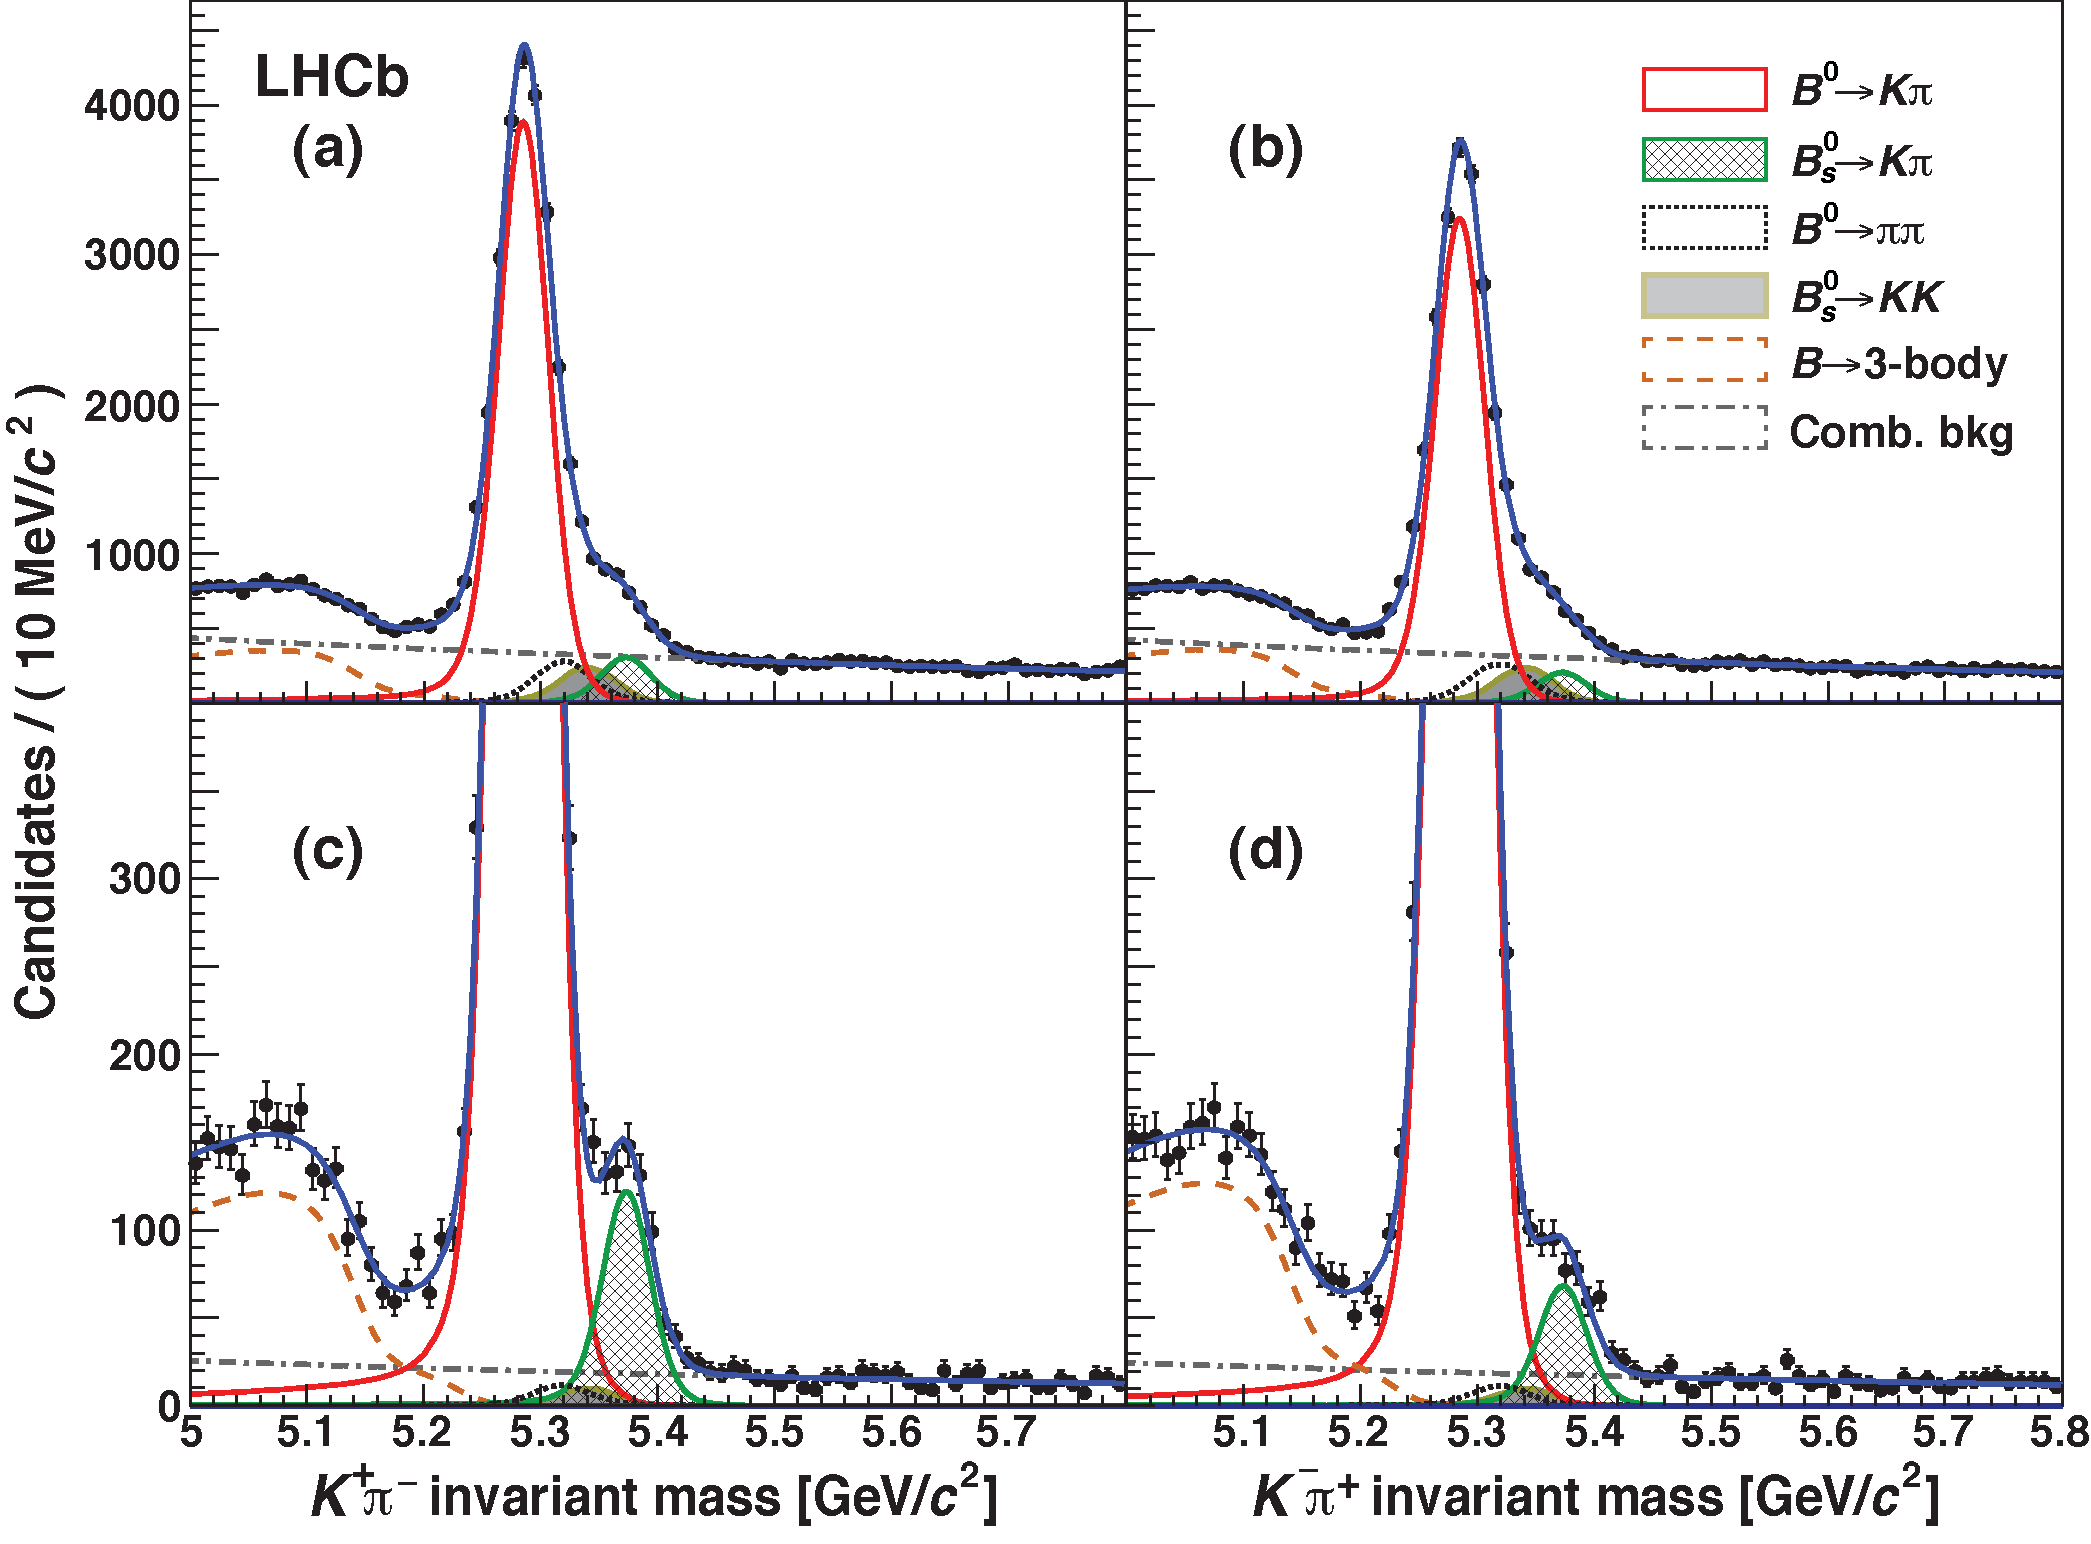
\includegraphics[width=0.8\textwidth]{03CPV/figs/DirectCPV.pdf}
	\caption{Invariant mass spectra for $A_{\CP}\left(\Bz\to\Kp\pim\right)$ (a,b) and $A_{\CP}\left(\Bs\to\Km\pip\right)$ (c,d). The figures (a) and (c) show the invariant mass distributions for \Kp\pim, figures (b) and (d) show the invariant mass distributions for \Km\pip.}
	\label{fig:DirectCPV}
\end{figure}


\subsection[head={Mixing \CP violation},tocentry={Mixing \CP violation}]{Mixing $\symbfsf{C{}P}$ violation}
\label{sec:MixingCPV}

Indirect \CP violation (\CP violation during mixing) means that the transition probabilities from a \Bz-meson to a \Bzb meson and vice versa are different.
As the name implies this type of \CP violation can only occur for neutral particles which can oscillate in their antiparticle.
Using the time evolution as shown in \cref{eq:timeEvolution} the probabilities of initially produced \Bz and \Bzb mesons to oscillate after a given time $t$ are
\begin{align}
% \left|\left<\Bz\Big|\Bz\!\left(t\right)\right>\right|^2=\frac{1}{4}
% \left(e^{-\Gamma_Ht}+e^{-\Gamma_Lt}+2e^{\frac{1}{2}\left(\Gamma_H+\Gamma_L\right)t}\cos\left(\dm t\right)\right),\\
\left|\left<\Bz\Big|\Bzb\!\left(t\right)\right>\right|^2=\frac{1}{4}\left|\frac{p}{q}\right|^2
\left(e^{-\Gamma_Ht}+e^{-\Gamma_Lt}-2e^{\frac{1}{2}\left(\Gamma_H+\Gamma_L\right)t}\cos\left(\dm t\right)\right),\\
\left|\left<\Bzb\Big|\Bz\!\left(t\right)\right>\right|^2=\frac{1}{4}\left|\frac{q}{p}\right|^2
\left(e^{-\Gamma_Ht}+e^{-\Gamma_Lt}-2e^{\frac{1}{2}\left(\Gamma_H+\Gamma_L\right)t}\cos\left(\dm t\right)\right).\\
% \left|\left<\Bzb\Big|\Bzb\!\left(t\right)\right>\right|^2=\frac{1}{4}
% \left(e^{-\Gamma_Ht}+e^{-\Gamma_Lt}+2e^{\frac{1}{2}\left(\Gamma_H+\Gamma_L\right)t}\cos\left(\dm t\right)\right).
\end{align}
Obviously to obtain the same probabilities $P(\Bz\to\Bzb)$ and $P(\Bzb\to\Bz)$
\begin{equation}
\left|\frac{q}{p}\right|=\left|\frac{p}{q}\right| \Rightarrow \left|\frac{q}{p}\right|=1
\end{equation}
is required.
Following \cref{eq:qoverp}, this implies that indirect \CP violation can only occur if the matrix elements $m_{12}$ and $\Gamma_{12}$ have different phases.
The \CP asymmetry for indirect \CP violation is defined as
\begin{equation}
A_{\CP}=\frac{\Gamma\left(\Bz\to\Bzb\right) - \Gamma\left(\Bzb\to\Bz\right)}{\Gamma\left(\Bz\to\Bzb\right) + \Gamma\left(\Bzb\to\Bz\right)}
= \frac{1-\left|\nicefrac{p}{q}\right|}{1+\left|\nicefrac{p}{q}\right|}
\end{equation}
The most prominent decay modes to measure \CP violation in mixing are semileptonic decays of neutral mesons.
This is due to the fact that semileptonc decays are usually flavour specific, \ie only the transition $\Bz\to\f$, but not $\Bz\to\fbar$ is allowed and thus the flavour of the meson at decay can be determined by the charge of the lepton in the final state.
For the \Bz and \Bs meson system \CP violation in mixing has been measured to be negligible \cite{HFLAV2016} what is in good agreement with the \ac{SM} predictions.

\subsection[head={Interference \CP violation},tocentry={Interference \CP violation}]{Interference $\symbfsf{C{}P}$ violation}
\label{sec:InterferenceCPV}

For this type of \CP violation we need to consider decays of \Bz and \Bzb mesons into a final state \f and its \CP-conjugate \fbar.
As was presented in the previous sections \CP violation arises from the clash between phases.
Indirect \CP violation arises if there is a clash between the phases of $m_{12}$ and $\Gamma_{12}$.
Inversely this means that \CP is conserved when there is phase $\xi$ such that
\begin{equation}
\begin{split}
m_{12}^\ast &= e^{2i\xi}m_{12}\\
\Gamma_{12}^\ast &= e^{2i\xi}\Gamma_{12}\label{eq:CPconservationMixing}
\end{split}
\end{equation}
what leads directly to $\nicefrac{q^2}{p^2} = e^{2i\xi}$ using \cref{eq:qoverp}.
Direct \CP violation on the other hand arises from a clash between the phases of two interfering decay amplitudes.
Considering the behaviour of the initial \Bz mesons
\begin{equation}
\CP\left|\Bz\right> =e^{i\xi}\left|\Bzb\right>\hspace{0.5cm}\text{and}\hspace{0.5cm}\CP\left|\Bzb\right>=e^{-i\xi}\left|\Bz\right>
\end{equation}
and of the final states
\begin{equation}
\CP\left|\f\right> =e^{i\xi_f}\left|\fbar\right>\hspace{0.5cm}\text{and}\hspace{0.5cm}\CP\left|\fbar\right>=e^{-i\xi_f}\left|\f\right>
\end{equation}
for the \CP conserving amplitudes the transformations can be expressed as
\begin{equation}
\begin{split}
\Abarfbar&=e^{i\left(\xi_f-\xi\right)}\Af,\\
\Afbar&=e^{i\left(\xi_f+\xi\right)}\Abarf. \label{eq:amplitudetransformation}
\end{split}
\end{equation}
After eliminating the phases the conditions $\left|\Af\right|=\left|\Abarfbar\right|$ and $\left|\Abarf\right|=\left|\Afbar\right|$ for \CP conservation in the decay directly follows. From \cref{eq:amplitudetransformation} one derives
\begin{equation}
\Af\Afbar=e^{2i\xi}\Abarfbar\Abarf
\end{equation}
what can be combined with \cref{eq:CPconservationMixing} and yields that \CP conservation implies
\begin{equation}
\arg\left(\frac{p^2}{q^2}\Af A_{\kern 1.5pt\overline{\kern -1.5pt f\kern 1.5pt}}^\ast\Afbar\overline{\kern -1.0pt A\kern -1.0pt}_{\kern 2.5pt\overline{\kern -1.5pt f\kern 1.5pt}}^\ast\right)=0.
\end{equation}
However to obtain this reasoning the \CP phase of the initial states transform and the phase of the off-diagonal matrix elements $m_{12}$ and $\Gamma_{12}$ were chosen to be equal.
If this would not be the case \CP would not be conserved in the interference of decay and decay after mixing.
Following this last type of \CP violation arises from a clash of the phase of $\nicefrac{q}{p}$ and the phase of the decay amplitude.

To investigate the effect on the decay rates of such processes it is useful to introduce first the following parameters:
\begin{equation}
\Lf=\frac{q}{p}\frac{\Abarf}{\Af}\hspace{0.5cm}\text{and}
\hspace{0.5cm}\Lfbar=\frac{p}{q}\frac{\Afbar}{\Abarfbar}.
\end{equation}
Using this parameters the conditions for \CP conervation simplify in the following way:
\begin{itemize}
	\item $\left|\Lf\right|=\left|\Lfbar\right| = 1$ means that \CP is conserved in decay and mixing
	\item However, even if the first condition is fullfilled $\mathcal{Im}\left(\Lf\right)\neq0$ or $\mathcal{Im}\left(\Lfbar\right)\neq0$ can hold. This means that in case of
	\begin{equation}
	\arg\left(\Lf\right)-\arg\left(\Lfbar\right)\neq0 \label{eq:conditionCPV}
	\end{equation}
	\CP violation may be present. Inverting this means that \CP conservation implies
	\begin{equation}
	\Lf=\frac{1}{\Lfbar}
	\end{equation}
\end{itemize}
Using then the time evolution presented in \cref{sec:TimeEvolution} the probability for the transitions $\left|\left<\,f\,\Big|T\Big|\Bz\!(t)\right>\right|^2$ can be calculated.
Here $\Bz\!(t)$ ($\Bzb\!(t)$) denotes a \B meson which was produced as a \Bz (\Bzb) at $t=0$:
\begin{align}
\left|\left<\,\f\,\Big|T\Big|\Bz\!(t)\right>\right|^2 =&
\left|\left<\,\f\,\Big|T\Big|\Bz\right>g_+-\frac{q}{p}\left<\,\f\,\Big|T\Big|\Bzb\right>g_-\right|^2\nonumber\\
=&\Af^2\left|g_+ - \frac{q}{p}\frac{\Abarf}{\Af} g_-\right|^2=\Af\left|g_+ -\Lf\,g_-\right|^2\nonumber\\
=&\Af^2\left(g_+g_+^*+\left|\Lf\right|^2g_-g_-^*-\left(\lambda_{f}^*g_-^*g_+ + \Lf\,g_+^* g_-\right)\right)
\end{align}
In analogy the probabilites for an initially produced \Bzb and a second finalstate \fbar are defined as
\begin{align}
\left|\left<\,\f\,\Big|T\Big|\Bzb\!(t)\right>\right|^2 &=
\Af^2\left|\frac{p}{q}\right|^2\left(g_+g_+^*\left|\Lf\right|^2+g_-g_-^*-\left(\Lfst g_+^*g_- + \Lf\,g_-^* g_+\right)\right)\\
\left|\left<\,\fbar\,\Big|T\Big|\Bz\!(t)\right>\right|^2 &=
\Abarfbar^2\left|\frac{q}{p}\right|^2\left(g_+g_+^*\left|\Lfbar\right|^2+g_-g_-^*-\left(\Lfbarst g_+^*g_- + \Lfbarst\,g_-^* g_+\right)\right)\\
\left|\left<\,\fbar\,\Big|T\Big|\Bzb\!(t)\right>\right|^2 &=
\Abarfbar^2\hphantom{\left|\frac{q}{p}\right|^2}\left(g_+g_+^*+\left|\Lfbar\right|^2g_-g_-^*-\left(\Lfbarst g_-^*g_+ + \Lfbar\,g_+^* g_-\right)\right)
\end{align}
Using
\begin{align}
g_{\pm}g_{\pm}^{*} &= \frac{1}{2}e^{-\Gamma t}\left(\cosh\left(\frac{\DG}{2}t\right)\pm\cos\left(\dm t\right)\right)\\
g_{\pm}^*g_{\mp} &=  \frac{1}{2}e^{-\Gamma t}\left(\sinh\left(\frac{\DG}{2}t\right)\mp i\sin\left(\dm t\right)\right)
\end{align}
the probabilities can be expressed as
\begin{align}
\left|\left<\,\f\,\Big|T\Big|\Bz\!(t)\right>\right|^2 =&
\frac{1}{2}e^{\Gamma t}\left|\Af\right|^2\left(1+\left|\Lf\right|^2\right)\hphantom{\left|\frac{p}{q}\right|^2}
\Bigg[\cosh\left(\frac{\DG}{2}t\right) + A_f^{\DG}\sinh\left(\frac{\DG}{2}t\right)\nonumber\\
&\hphantom{\frac{1}{2}e^{\Gamma t}\left|\Af\right|^2\left(1+\left|\Lf\right|^2\right)\left|\frac{p}{q}\right|^2\Bigg[}
-\Sf\sin\left(\dm t\right)+\Cf\cos\left(\dm t\right)\Bigg]\\
\left|\left<\,\f\,\Big|T\Big|\Bzb\!(t)\right>\right|^2 =&
\frac{1}{2}e^{\Gamma t}\left|\Af\right|^2\left(1+\left|\Lf\right|^2\right)\left|\frac{p}{q}\right|^2
\Bigg[\cosh\left(\frac{\DG}{2}t\right) + A_f^{\DG}\sinh\left(\frac{\DG}{2}t\right)\nonumber\\
&\hphantom{\frac{1}{2}e^{\Gamma t}\left|\Af\right|^2\left(1+\left|\Lf\right|^2\right)\left|\frac{p}{q}\right|^2\Bigg[}
+\Sf\sin\left(\dm t\right)-\Cf\cos\left(\dm t\right)\Bigg]\\
\left|\left<\,\fbar\,\Big|T\Big|\Bz\!(t)\right>\right|^2 =&
\frac{1}{2}e^{\Gamma t}\left|\Abarfbar\right|^2\left(1+\left|\Lfbar\right|^2\right)\left|\frac{q}{p}\right|^2
\Bigg[\cosh\left(\frac{\DG}{2}t\right) + A_{\kern 1.5pt\overline{\kern -1.5pt f\kern 1.5pt}}^{\DG}\sinh\left(\frac{\DG}{2}t\right)\nonumber\\
&\hphantom{\frac{1}{2}e^{\Gamma t}\left|\Af\right|^2\left(1+\left|\Lf\right|^2\right)\left|\frac{q}{p}\right|^2\Bigg[}
-\Sfbar\sin\left(\dm t\right)+\Cfbar\cos\left(\dm t\right)\Bigg]\\
\left|\left<\,\fbar\,\Big|T\Big|\Bzb\!(t)\right>\right|^2 =&
\frac{1}{2}e^{\Gamma t}\left|\Abarfbar\right|^2\left(1+\left|\Lfbar\right|^2\right)\hphantom{\left|\frac{q}{p}\right|^2}
\Bigg[\cosh\left(\frac{\DG}{2}t\right) + A_{\kern 1.5pt\overline{\kern -1.5pt f\kern 1.5pt}}^{\DG}\sinh\left(\frac{\DG}{2}t\right)\nonumber\\
&\hphantom{\frac{1}{2}e^{\Gamma t}\left|\Af\right|^2\left(1+\left|\Lf\right|^2\right)\left|\frac{q}{p}\right|^2\Bigg[}
+\Sfbar\sin\left(\dm t\right)-\Cfbar\cos\left(\dm t\right)\Bigg]
\end{align}
with the \CP coefficients
\begin{align}
A_f^{\DG}&=-\frac{2\mathcal{Re}\left(\Lf\right)}{1+\left|\Lf\right|^2}\hspace{0.5cm}
\Sf=\frac{2\mathcal{Im}\left(\Lf\right)}{1+\left|\Lf\right|^2}\hspace{0.5cm}
\Cf=\frac{1-\left|\Lf\right|^2}{1+\left|\Lf\right|^2}\\
A_{\kern 1.5pt\overline{\kern -1.5pt f\kern 1.5pt}}^{\DG}&=-\frac{2\mathcal{Re}\left(\Lfbar\right)}{1+\left|\Lfbar\right|^2}\hspace{0.5cm}
\Sfbar=-\frac{2\mathcal{Im}\left(\Lfbar\right)}{1+\left|\Lfbar\right|^2}\hspace{0.5cm}
\Cfbar=-\frac{1-\left|\Lfbar\right|^2}{1+\left|\Lfbar\right|^2}.
\end{align}
This type of \CP violation has been measured by the \B-factories \belle and \babar, as well as by \lhcb.
The most prominent analysis is probably the measurement of $\sin\left(2\beta\right)$ in the so-called golden mode \BdToJPsiKS \cite{Aaij:2015vza}.
As both \Bz mesons reach the same finalstate \f $\Lfbar=-\Lf$ holds and the condition in \cref{eq:conditionCPV} can be reduced to $\arg\left(\Lf\right)\neq0$.
The \CP asymmetry in this case is defined as
\begin{equation}
A_{\CP}(t)=\frac{\Gamma\left(\BdToJPsiKS\right)}{\Gamma\left(\BdToJPsiKS\right)}=\Sf\sin\left(\dmd t\right)+\Cf\cos\left(\dmd t\right)
\end{equation}
As in this case $\Cf=0$ is expected the a sine oscillation is expected as can be seen in \cref{fig:sin2beta}.
\begin{figure}[tbp]
	\centering
	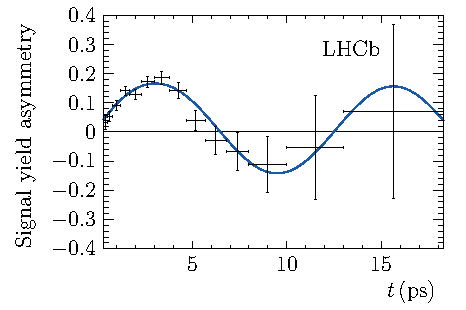
\includegraphics[width=0.6\textwidth]{03CPV/figs/InterferenceCPV.pdf}
	\caption{Time-dependent signal yield asymmetry $\left(N_{\Bzb}-N_{\Bz}\right)/\left(N_{\Bzb}-N_{\Bz}\right)$. The black points represent the used datasample, the solid curve is the projection of the signal \PDF.}
	\label{fig:sin2beta}
\end{figure}
